\documentclass[12pt, letterpaper]{article}
\usepackage[margin=1in]{geometry}
\usepackage{amsmath, amssymb}
\usepackage{graphicx}
\usepackage{natbib}
\usepackage{hyperref}
\usepackage{booktabs}

\newcommand{\hmpc}{\,h^{-1}\,\mathrm{Mpc}}
\newcommand{\hkpc}{\,h^{-1}\,\mathrm{kpc}}
\newcommand{\arcminsq}{\,\mathrm{arcmin}^{-2}}
\newcommand{\lam}{\lambda}
\newcommand{\zlam}{z_\lambda}

\title{Cluster Member Galaxy Angular Density vs.\ Fiber Density:\\
       Implications for Spectroscopic Completeness in Stage-V Surveys}
\author{Spec-S5 White Paper --- Working Draft}
\date{\today}

\begin{document}
\maketitle

% ------------------------------------------------------------------
\section{Motivation}
\label{sec:motivation}
% ------------------------------------------------------------------

Multi-object fiber spectrographs allocate a finite number of fibers over
a fixed field of view, setting an effective \emph{fiber density}
(targets\,$\arcminsq$).  When the projected angular density of cluster
member galaxies exceeds this fiber density, a single-pass observation
cannot obtain spectra for all members simultaneously; multi-pass
strategies or fiber-priority schemes become necessary.

This note quantifies the member-galaxy angular density for a
well-characterized, low-redshift cluster sample and compares it with the
fiber densities of two representative spectroscopic surveys:
\begin{itemize}
    \item \textbf{DESI}: ${\sim}\,5{,}000$ fibers over a
          $7\;\mathrm{deg}^2$ field of view
          $\Rightarrow 0.198\arcminsq$;
    \item \textbf{Stage-V (Spec-S5)}: ${\sim}\,20{,}000$ fibers over a
          $5\;\mathrm{deg}^2$ field of view
          $\Rightarrow 1.111\arcminsq$.
\end{itemize}
Understanding where the cluster angular density falls relative to these
thresholds informs whether satellite galaxy spectroscopic redshifts can
be obtained ``for free'' during the primary survey or whether dedicated
multi-pass observations are required.

% ------------------------------------------------------------------
\section{Data}
\label{sec:data}
% ------------------------------------------------------------------

We use the SDSS DR8 red-sequence Matched-filter Probabilistic
Percolation (redMaPPer) cluster catalog \citep{Rykoff2014}:
\begin{itemize}
    \item \textbf{Cluster catalog} (\texttt{redmapper\_sdss\_dr8.fit}):
          cluster ID, photometric redshift $\zlam$, and richness $\lam$.
    \item \textbf{Member catalog} (\texttt{redmapper\_sdss\_dr8\_mem.fit}):
          member galaxy ID, parent cluster ID, and projected
          cluster-centric distance $R$ in units of $\hmpc$.
\end{itemize}
Both catalogs are publicly available through VizieR
(J/ApJ/785/104, Tables~1 and~2).
We restrict the analysis to clusters at $\zlam \leq 0.5$, yielding
23{,}801 clusters.

% ------------------------------------------------------------------
\section{Method}
\label{sec:method}
% ------------------------------------------------------------------

\subsection{Angular density definition}

For each cluster we compute a projected angular density
$\Sigma_\theta$ as:
\begin{equation}
    \Sigma_\theta
    = \frac{N}{\pi\,\theta_{\max}^2}
    \quad [\arcminsq],
    \label{eq:density}
\end{equation}
where $N$ is the number of member galaxies (or the richness $\lam$)
and $\theta_{\max}$ is the angular radius corresponding to the maximum
projected distance $R_{\max}$ among the members.

\subsection{Physical-to-angular conversion}

The member distances $R$ are given in $\hmpc$ units.  We convert to
physical Mpc using $R_{\rm phys} = R / h$ with $h = 0.7$, and then to an
angular separation via:
\begin{equation}
    \theta = \frac{R_{\rm phys}}{d_A(z)},
    \label{eq:theta}
\end{equation}
where $d_A(z)$ is the angular diameter distance computed under a flat
$\Lambda$CDM cosmology with $H_0 = 70\;\mathrm{km\,s^{-1}\,Mpc^{-1}}$
and $\Omega_m = 0.3$.  The result is converted from radians to arcmin.

\subsection{Numerator choices: raw count vs.\ richness}

We compute two versions of Equation~\ref{eq:density}:
\begin{enumerate}
    \item $N = N_{\rm mem}$, the raw number of members listed in the
          member catalog for each cluster;
    \item $N = \lam$, the redMaPPer richness, which applies statistical
          corrections for background contamination and membership
          probability weighting.
\end{enumerate}

\subsection{Radial decomposition: inner vs.\ outer}

To assess whether fiber contention is concentrated in cluster cores, we
split each cluster's members at a projected radius of
$R_{\rm split} = 150\hkpc$ ($= 0.15\hmpc$):
\begin{itemize}
    \item \textbf{Inner region} ($R \leq R_{\rm split}$):
          $\Sigma_{\rm inner} = N_{\rm inner}\,/\,(\pi\,\theta_{\rm split}^2)$.
    \item \textbf{Outer region} ($R > R_{\rm split}$):
          $\Sigma_{\rm outer} = N_{\rm outer}\,/\,
          \bigl[\pi\,(\theta_{\rm max,outer}^2 - \theta_{\rm split}^2)\bigr]$,
          where $\theta_{\rm max,outer}$ is the angular radius
          corresponding to the maximum $R$ among outer members.
\end{itemize}
Here, $\theta_{\rm split}$ is the angular equivalent of $R_{\rm split}$
at the cluster redshift (Equation~\ref{eq:theta}).

% ------------------------------------------------------------------
\section{Results}
\label{sec:results}
% ------------------------------------------------------------------

\subsection{Total angular density}

Table~\ref{tab:summary} summarizes the median angular densities across
all 23{,}801 clusters.  The raw-count density ($N_{\rm mem}$-based)
exceeds the richness-based density because the member catalog includes
galaxies that survive the initial selection but carry membership
probability $< 1$ and would be down-weighted in $\lam$.

\begin{table}[h]
\centering
\caption{Median member galaxy angular densities for redMaPPer SDSS DR8
         clusters at $\zlam \leq 0.5$.}
\label{tab:summary}
\begin{tabular}{lc}
\toprule
Density estimator & Median $[\arcminsq]$ \\
\midrule
Total ($N_{\rm mem}$)               & 1.14 \\
Total ($\lam$)                      & 0.71 \\
Inner ($R \leq 150\hkpc$)           & 4.19 \\
Outer ($R > 150\hkpc$)              & 0.99 \\
\midrule
DESI fiber density                  & 0.20 \\
Stage-V fiber density               & 1.11 \\
\bottomrule
\end{tabular}
\end{table}

\subsection{Redshift dependence}

Figure~\ref{fig:total} shows the angular density as a function of
cluster redshift.  Both the $N_{\rm mem}$-based and $\lam$-based
densities rise steeply from $z \sim 0.05$ to $z \sim 0.2$--$0.3$ and
flatten at higher redshift.  This behavior is driven by the shrinking
angular diameter distance: at higher redshift, the same physical extent
subtends a smaller angle, compressing members into a smaller angular
area.

Nearly all clusters lie above the DESI fiber density threshold at all
redshifts.  The Stage-V threshold intersects the bulk of the
distribution, with most clusters above it for $z \gtrsim 0.15$ in the
$N_{\rm mem}$ case and $z \gtrsim 0.25$ in the $\lam$ case.

\begin{figure}[ht]
\centering
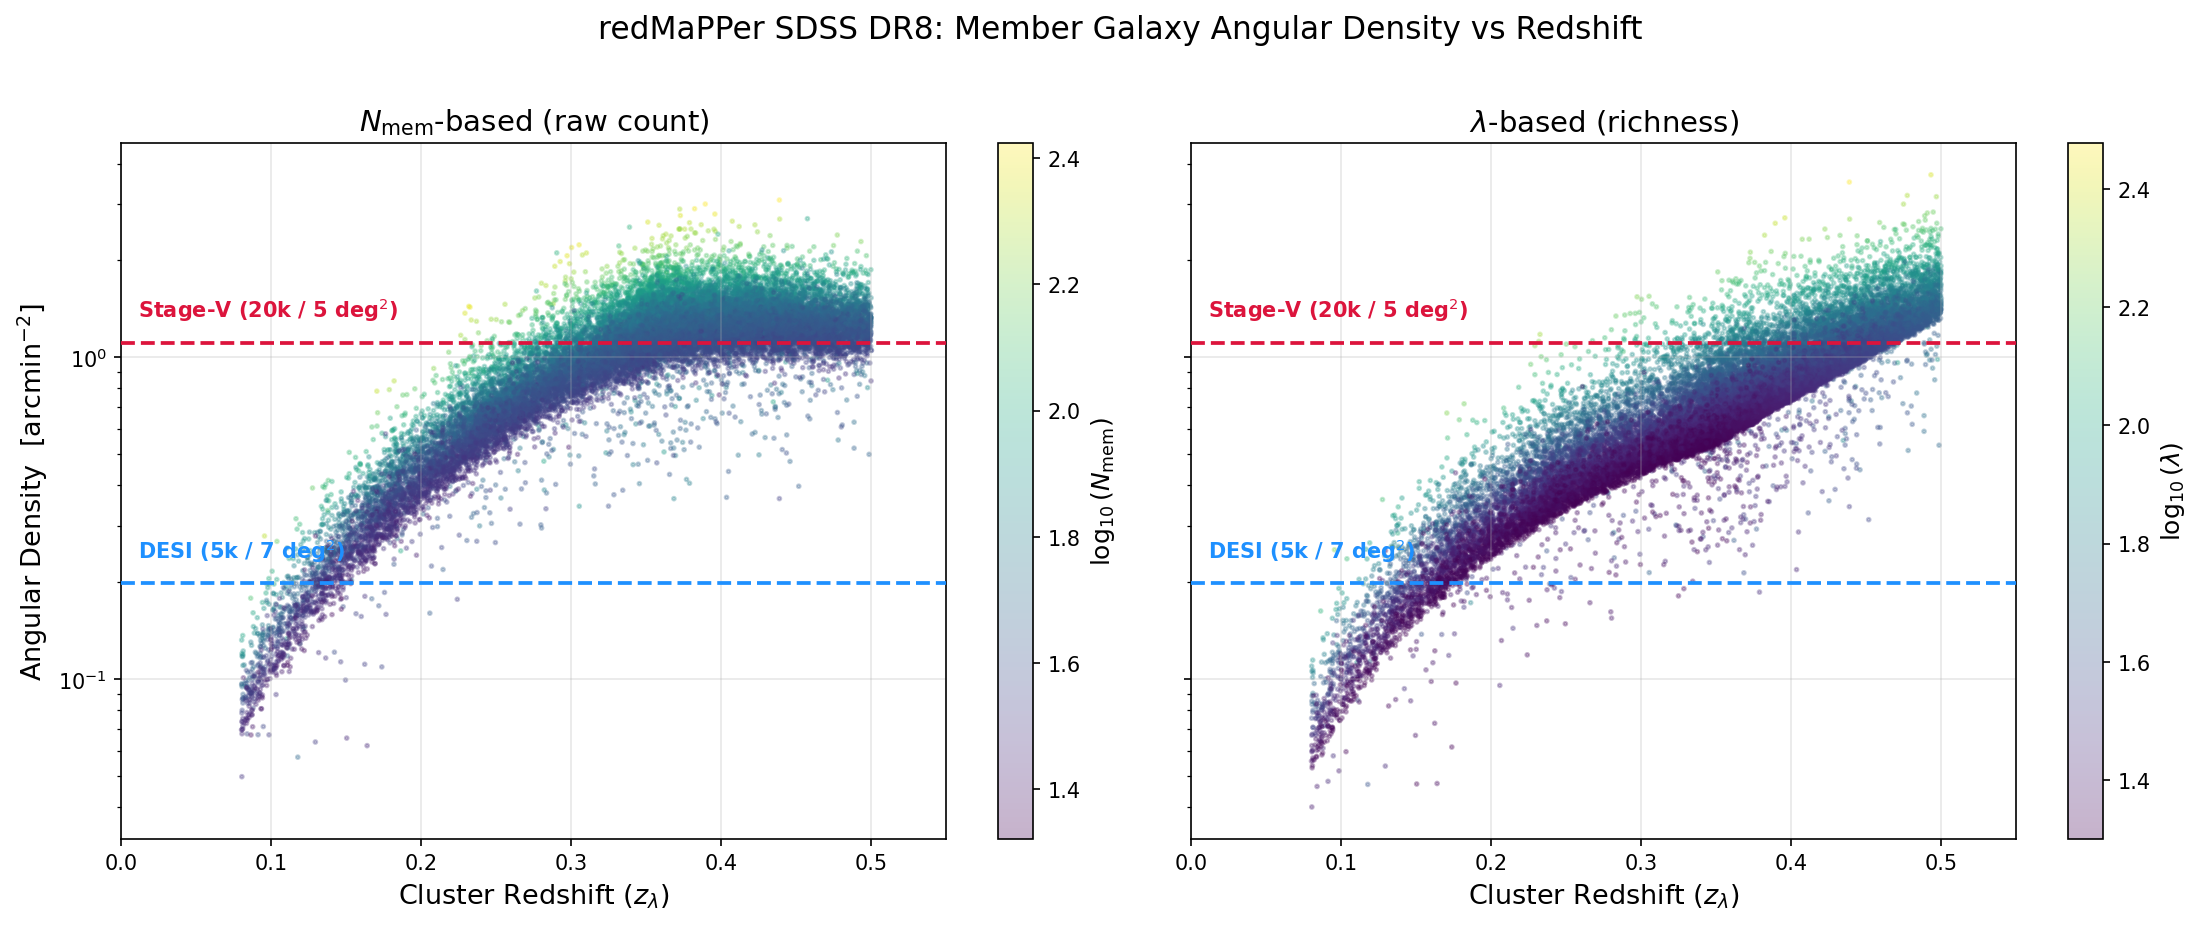
\includegraphics[width=\textwidth]{figures/angular_density_vs_redshift.png}
\caption{Cluster member galaxy angular density vs.\ photometric
         redshift $\zlam$ for 23{,}801 redMaPPer SDSS DR8 clusters.
         \emph{Left}: using the raw member count $N_{\rm mem}$.
         \emph{Right}: using the richness $\lam$.
         Color encodes the log of the numerator.
         Horizontal dashed lines mark the DESI (blue; $0.198\arcminsq$)
         and Stage-V (red; $1.111\arcminsq$) fiber densities.}
\label{fig:total}
\end{figure}

\subsection{Inner vs.\ outer regions}

Figure~\ref{fig:inner_outer} compares the inner and outer angular
densities.  The inner 150$\hkpc$ core has a median density of
$4.19\arcminsq$, roughly $4\times$ higher than the outer annulus
($0.99\arcminsq$).  The inner density exceeds both the DESI and
Stage-V fiber densities across essentially the entire redshift range,
confirming severe fiber contention in cluster cores even for Stage-V.

The outer region is more favorable: its density falls between the DESI
and Stage-V thresholds for many low-redshift clusters ($z \lesssim 0.15$)
and rises above the Stage-V line at $z \gtrsim 0.2$--$0.3$.  This
indicates that a single-pass Stage-V observation can achieve high
spectroscopic completeness for \emph{outer} satellite galaxies at
$z \lesssim 0.2$, but multi-pass strategies become necessary at higher
redshifts or for core regions.

\begin{figure}[ht]
\centering
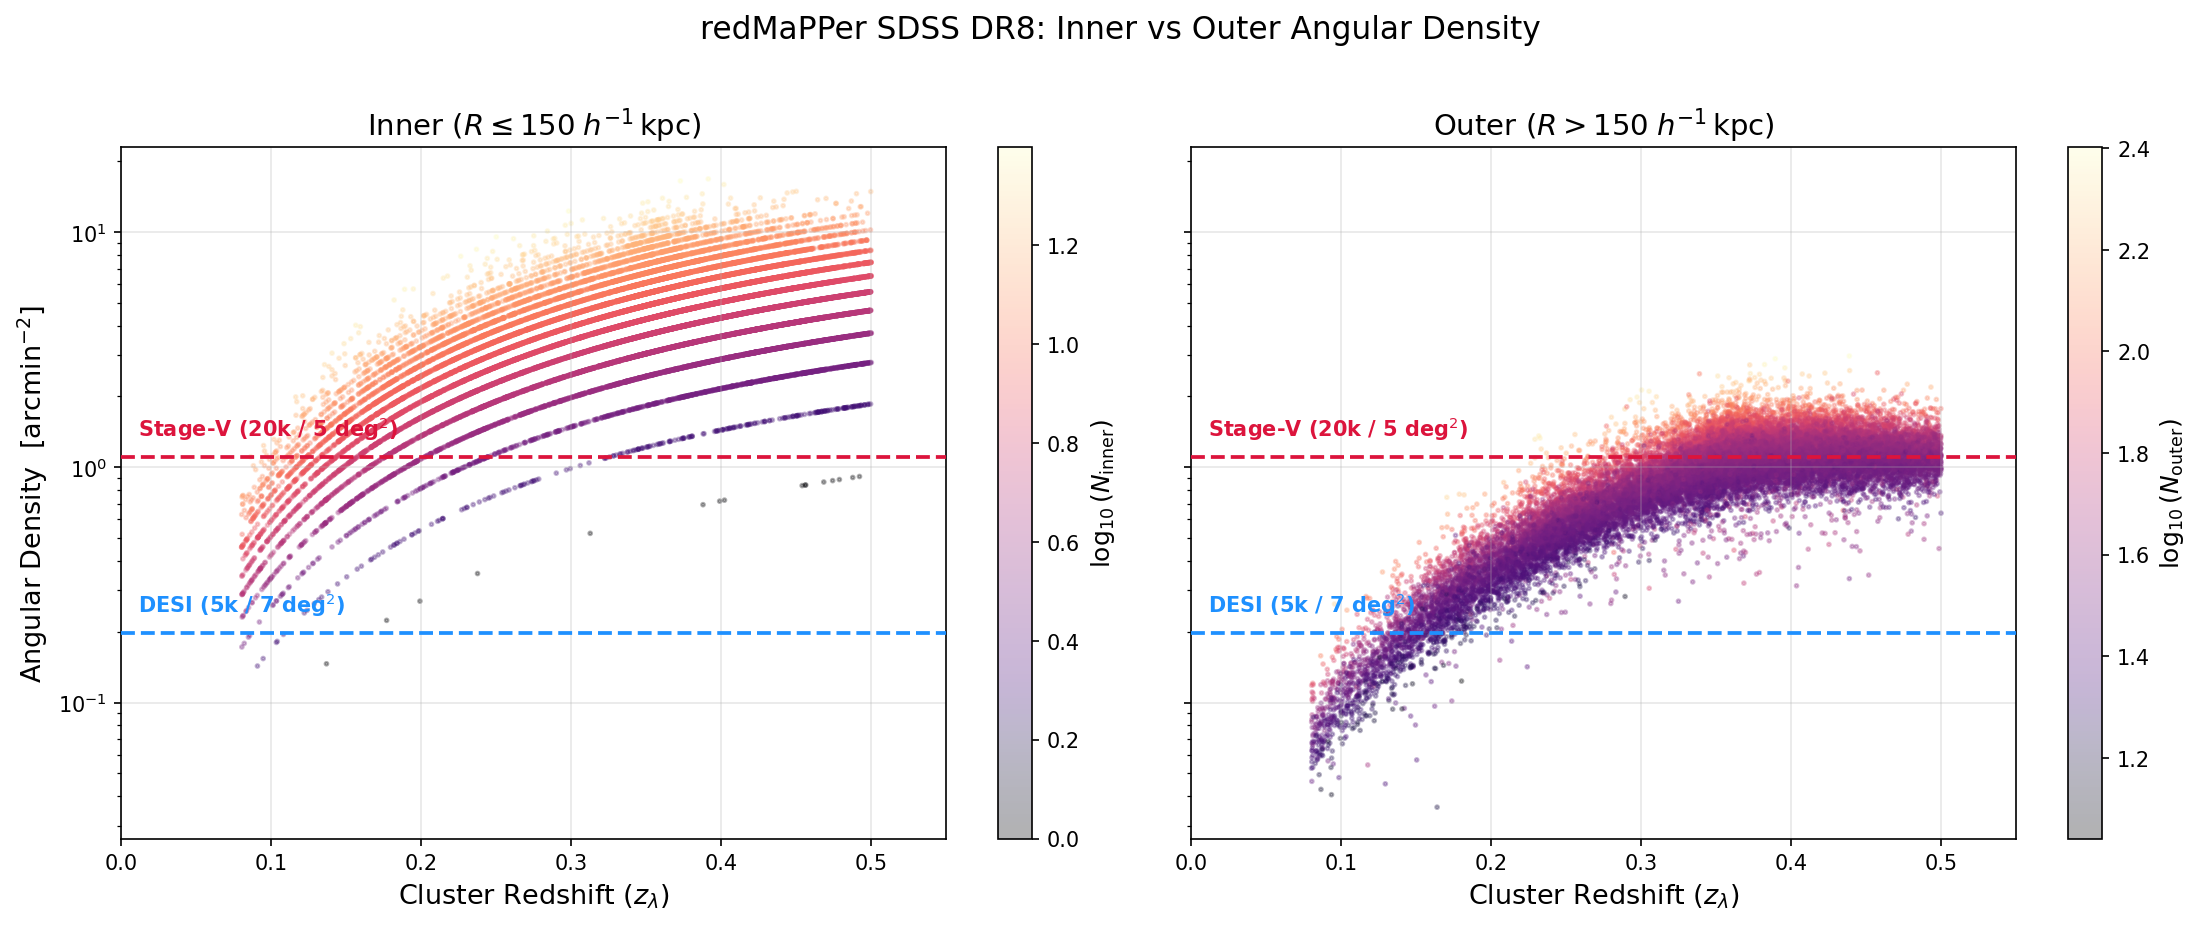
\includegraphics[width=\textwidth]{figures/angular_density_inner_outer.png}
\caption{Inner vs.\ outer angular density for the same cluster sample.
         \emph{Left}: inner region ($R \leq 150\hkpc$).
         \emph{Right}: outer annulus ($R > 150\hkpc$).
         Color encodes the log of the member count in each region.
         Survey fiber density thresholds are shown as in
         Figure~\ref{fig:total}.}
\label{fig:inner_outer}
\end{figure}

% ------------------------------------------------------------------
\section{Discussion}
\label{sec:discussion}
% ------------------------------------------------------------------

These results have several implications for the Spec-S5 survey design:

\begin{enumerate}
    \item \textbf{Core completeness requires multi-pass.}  The inner
          $150\hkpc$ of clusters is ${\sim}\,4\times$ denser than the
          Stage-V fiber density at all redshifts.  Achieving high
          spectroscopic completeness in cores will require either
          multiple passes or dedicated cluster-mode observations.

    \item \textbf{Outskirts are accessible in single-pass at low $z$.}
          For $z \lesssim 0.2$, the outer angular density falls near or
          below the Stage-V fiber density, meaning that satellite
          spectroscopic redshifts in cluster outskirts can largely be
          obtained ``for free'' during the primary survey.

    \item \textbf{Richness vs.\ raw counts.}  The $\lam$-based density
          is ${\sim}\,40\%$ lower than the raw-count density, reflecting
          background subtraction.  Since the actual targets for fiber
          assignment are \emph{candidate} members (not yet background-
          subtracted), the raw-count density is the more operationally
          relevant metric for fiber-allocation planning.

    \item \textbf{Redshift-dependent strategy.}  A natural survey
          strategy would be to rely on single-pass for
          $z \lesssim 0.2$ clusters and allocate additional passes for
          higher-redshift systems where the angular density exceeds the
          fiber density across the full radial extent.
\end{enumerate}

% ------------------------------------------------------------------
\section{Reproducibility}
\label{sec:reproducibility}
% ------------------------------------------------------------------

The analysis is implemented in a single Python script
(\texttt{angular\_density.py}) using \texttt{astropy} (FITS I/O and
cosmological calculations), \texttt{numpy}, and \texttt{matplotlib}.
The cosmological model is flat $\Lambda$CDM with
$(H_0,\,\Omega_m) = (70,\, 0.3)$.  All per-cluster results (ID,
redshift, member counts, angular sizes, and densities for total, inner,
and outer regions) are saved to \texttt{angular\_density\_results.dat}.

\bibliographystyle{aasjournal}
\begin{thebibliography}{1}
\bibitem[Rykoff et al.(2014)]{Rykoff2014}
Rykoff, E.~S., Rozo, E., Busha, M.~T., et al.\ 2014,
\href{https://doi.org/10.1088/0004-637X/785/2/104}{ApJ, 785, 104}
\end{thebibliography}

\end{document}
